\documentclass[10pt,aspectratio=169]{beamer}
\usetheme{default}
\usecolortheme{seagull}
\setbeamertemplate{navigation symbols}{}
\setbeamertemplate{footline}[frame number]
\setbeamerfont{frametitle}{series=\bfseries,size=\large}
\setbeamercolor{frametitle}{fg=black!85}
\setbeamercolor{structure}{fg=black!70}
\usepackage{booktabs}
\usepackage{xcolor}
\definecolor{okblue}{HTML}{0072B2}
\definecolor{okorange}{HTML}{E69F00}
\definecolor{okred}{HTML}{D55E00}
\definecolor{okgreen}{HTML}{009E73}
\newcommand{\good}[1]{\textcolor{okgreen}{#1}}
\newcommand{\bad}[1]{\textcolor{okred}{#1}}

\title{\textbf{MX17 drift window \& drift voltage}\\
\large measurement-driven sizing of the DREAM readout for beam data}
\author{Dylan Neff}
\date{2026-07-19 \quad (run\_54 cosmics + run\_55 beam, nTOF EAR2)}

\begin{document}

\begin{frame}
  \titlepage
  \vfill
  \centering\small
  \textbf{TL;DR:}\; latency $35\to\mathbf{32}$,\; n\_samples $32\to\mathbf{28}$,\;
  det~A drift $600\to\mathbf{700}$~V (staged),\; B/C/D stay 800~V,\;
  short on-beam det-A drift scan as the 700~V spark gate.
\end{frame}

\begin{frame}{The question and the constraints}
  \begin{columns}[T]
    \column{0.55\textwidth}
    \textbf{Decide for the 4-det Micromegas stack:}
    \begin{itemize}
      \item minimum \texttt{n\_samples} (60 ns DREAM sampling) with no drifting primary lost on \emph{any} detector;
      \item drift HV: det A spark-limited (sparked @800 V, stable @600 V) --- push to 700?
    \end{itemize}
    \vspace{0.5em}
    \textbf{Hard facts}
    \begin{itemize}
      \item 30 mm gap, Ar/iC$_4$H$_{10}$ 90/10, all four dets;
      \item \textbf{series gas line A$\to$B$\to$C$\to$D} (wetness rises down-chain);
      \item current: 32 smp $\times$ 60 ns = 1.92 µs, latency 35;
      \item drift: A 600 V, B/C/D 800 V; resist 560 V.
    \end{itemize}
    \column{0.42\textwidth}
    \textbf{Data used (2026-07-18)}
    \begin{itemize}
      \item run\_54: cosmics, 4 subruns, 9k evts/FEU;
      \item \textbf{run\_55: beam} (19:11, Mode-3 scint-doubles, r560 subruns) --- real trigger, real flash;
      \item Magboltz: clean 90/10 @CERN P + H$_2$O grid.
    \end{itemize}
    \vspace{0.5em}
    \small June lesson: wet gas (${\sim}1\%$ H$_2$O) \emph{halves} low-field drift speed; the 500 V June point truncated its window.
  \end{columns}
\end{frame}

\begin{frame}{Method: de-noising is the whole game}
  \begin{columns}[T]
    \column{0.47\textwidth}
    \textbf{Extractor} (\texttt{24\_drift\_time\_edges.py})
    \begin{itemize}
      \item common mode per 64-ch DREAM chip (noise is per-connector), 2 iterations, track strips masked;
      \item per-strip robust MAD threshold + width $\geq$2, hot-channel mask;
      \item spatial clusters ($\geq$3 adjacent strips) = track;
      \item per event: prompt (earliest peak), deep edge (latest peak), pulse rise/end, span.
    \end{itemize}
    \vspace{0.4em}
    \textbf{The decisive cut:} events with $>$100 hit strips (``monster''/flash, $\sim$2\% of beam triggers; det-D sparks in cosmics) are excluded.
    \column{0.5\textwidth}
    \centering
    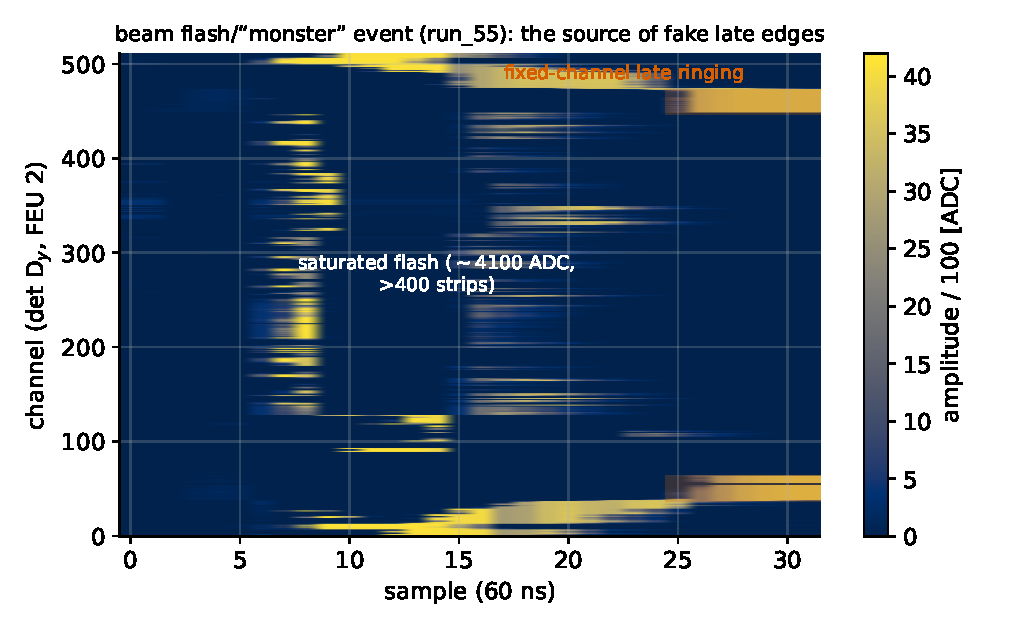
\includegraphics[width=\textwidth]{fig_flash.pdf}
  \end{columns}
\end{frame}

\begin{frame}{Finding 1 --- the ``slow/late B \& D'' of the first look was artifact}
  \begin{itemize}
    \item Saturated flash events are followed by \textbf{fixed channel blocks} (e.g.\ FEU2 ch 38--63, 448--472) ringing at samples 24--31 $\Rightarrow$ they masqueraded as 25-strip ``late clusters''. Every inspected late cluster was one of these.
    \item det D cosmics: 129--152 spark events / 9000 $\Rightarrow$ after the cut, D$_x$ ceiling fraction \bad{8.9\%} $\to$ \good{1.5\%}.
    \item det B looks contaminated only in the cosmic run (coherent noise); its \emph{beam} x-plane matches C/D. No evidence B is slow.
  \end{itemize}
  \vspace{0.4em}
  \centering
  \begin{tabular}{lcccc}
    \toprule
    ceiling fraction (peak $\geq$ smp 31) & A$_x$ & C$_x$ & D$_x$ & B$_x$ \\
    \midrule
    raw first look (handoff) & 0.3\% & 0.6\% & \bad{7--20\%} & \bad{21--30\%} \\
    de-noised + monster cut (cosmics) & \good{0.3\%} & \good{0.4\%} & \good{1.5\%} & (noise-limited)\\
    \bottomrule
  \end{tabular}
  \vspace{0.6em}
  \begin{block}{}
    \centering \textbf{No detector is losing drifting primaries at 32 smp / latency 35 today.}
  \end{block}
\end{frame}

\begin{frame}{Finding 2 --- timing is universal: prompt at sample 8--9, both triggers}
  \centering
  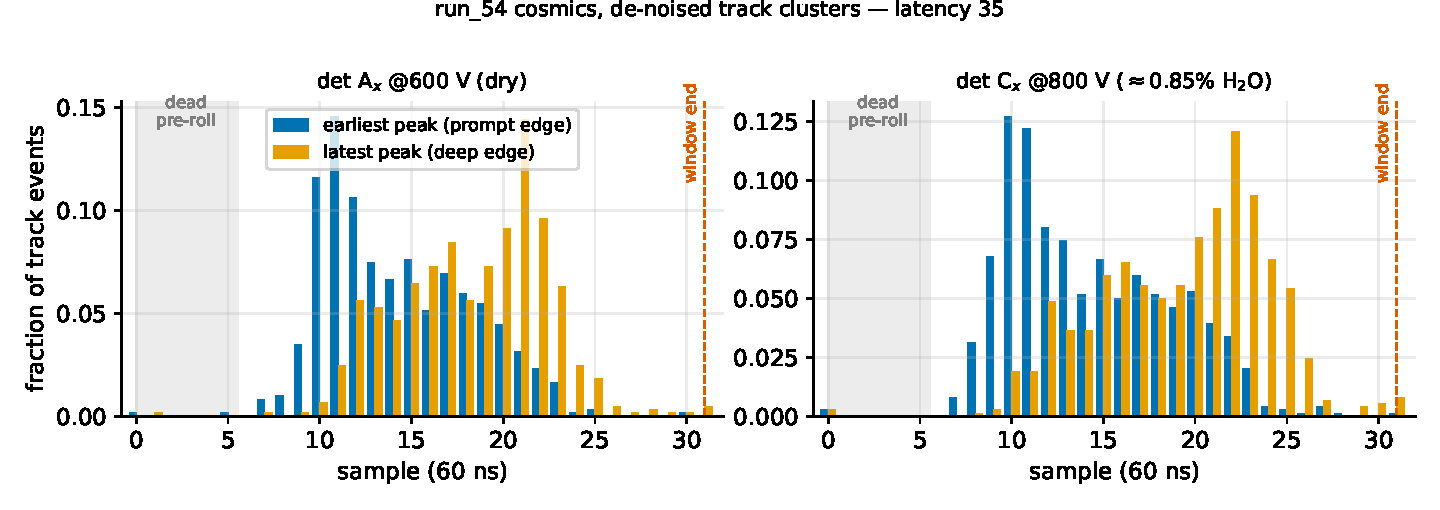
\includegraphics[width=0.9\textwidth]{fig_hist.pdf}
  \begin{itemize}
    \item First signal above threshold: sample 6--7 (p5); prompt \emph{peak}: 8--9 $\Rightarrow$ peak $\approx$ latency$-$26.
    \item Identical in cosmic-singles and beam Mode-3 triggers, all four detectors --- the suspected per-detector $t_0$ offsets were cluster-geometry artifacts. \textbf{One latency serves both run types.}
    \item \bad{These are PEAK positions.} The pulse has width --- it rises 4 smp before the peak and falls $+$7 smp after (next slide). The window must hold the rise (with baseline) AND the fall, not just the peaks.
  \end{itemize}
\end{frame}

\begin{frame}{Pulse footprint --- the window must hold rise + peak + fall}
  \begin{columns}[T]
    \column{0.6\textwidth}
    \centering
    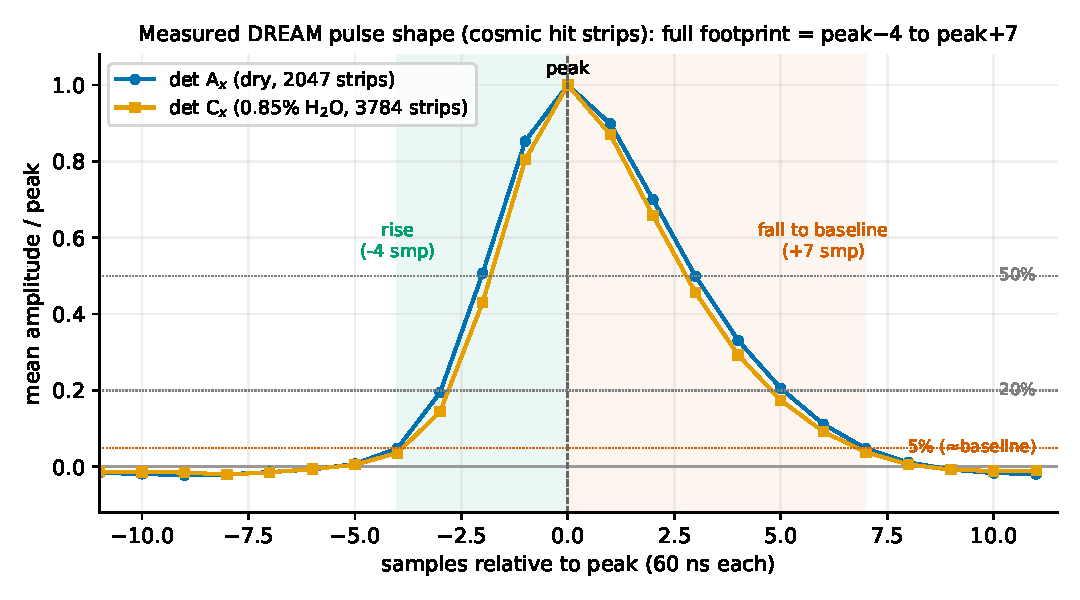
\includegraphics[width=\textwidth]{fig_pulse_shape.pdf}
    \column{0.38\textwidth}
    \small Peak-aligned mean pulse (cosmic hit strips, A$_x$ \& C$_x$ identical):
    \begin{itemize}\small
      \item rise onset (5\%) at \textbf{peak$-$4}; want $\sim$3 baseline before it.
      \item fall to 20\% at \textbf{peak$+$5}; to baseline (5\%) at \textbf{peak$+$7}.
    \end{itemize}
    \vspace{0.4em}
    A primary spans \textbf{$\sim$11 smp} (peak$-$4 $\to$ peak$+$7). \bad{The earlier ``+2 fall'' was wrong by $\sim$5 smp} --- that is what moves the trim from n=28 back to n=30.
  \end{columns}
\end{frame}

\begin{frame}{Finding 3 --- water: A is dry; B, C, D all breathe ${\sim}0.8$\% H$_2$O}
  \begin{columns}[T]
    \column{0.52\textwidth}
    \centering
    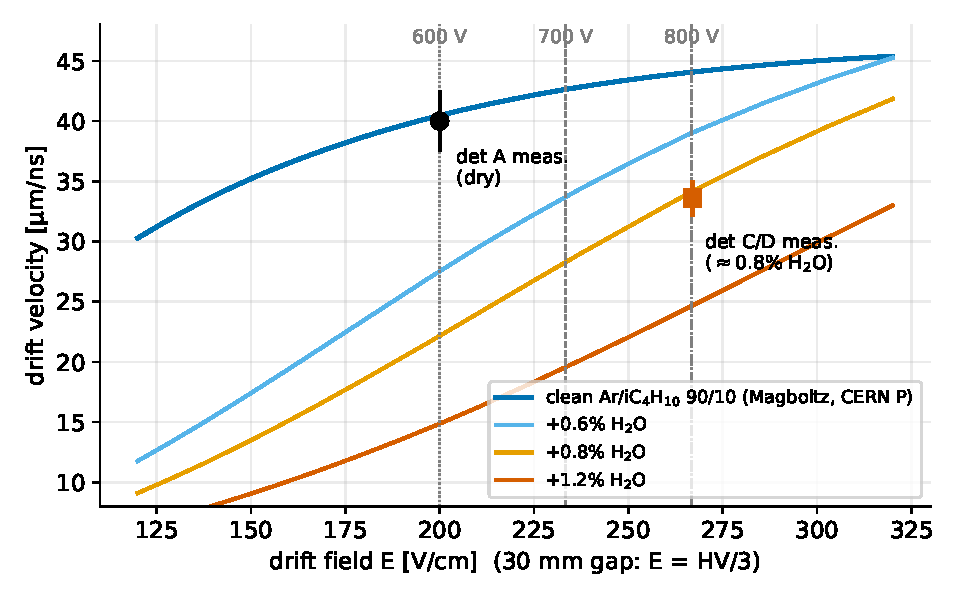
\includegraphics[width=\textwidth]{fig_ve.pdf}
    \column{0.45\textwidth}
    \small
    Span of $\geq$6-strip clusters (cosmics, p95), recorded-column fraction 0.89 anchored on det A = clean:
    \vspace{0.3em}
    \begin{tabular}{lcccc}
      \toprule
      det & HV & $T_{\rm full}$ & $v$ & H$_2$O \\
       & [V] & [smp] & [µm/ns] & \\
      \midrule
      A & 600 & 12.4 & $\approx$40 & \good{$\leq$0.2\%} \\
      C & 800 & 15.2 & 33.0 & \bad{0.85\%} \\
      D & 800 & 14.6 & 34.2 & \bad{0.80\%} \\
      B & 800 & $\sim$15 & $\sim$33 & \bad{$\sim$0.8\%} \\
      \bottomrule
    \end{tabular}
    \vspace{0.6em}
    \begin{itemize}
      \item Chain wetting \textbf{saturates at the first hop}: no A$\to$D slope, B$\approx$C$\approx$D near June's $\sim$1\% equilibrium.
      \item Deep-charge attenuation mild: $\lambda_{\rm eff}\approx$ 23--25 mm (June: 16--18).
    \end{itemize}
  \end{columns}
\end{frame}

\begin{frame}{Window budget (measured pulse footprint)}
  \centering
  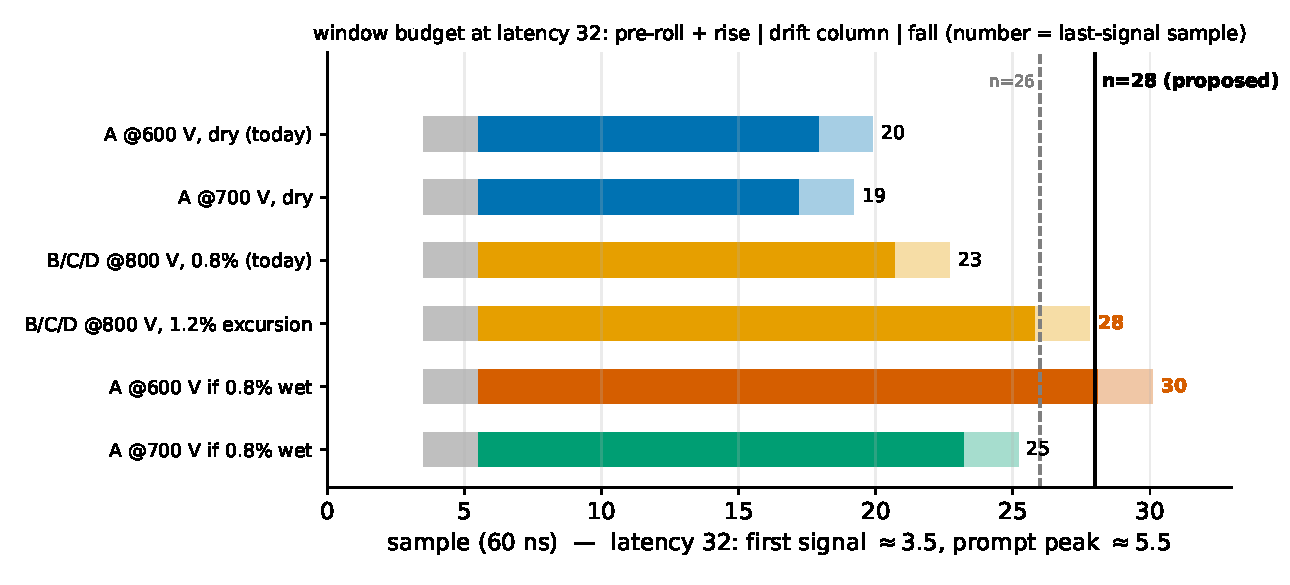
\includegraphics[width=0.82\textwidth]{fig_budget.pdf}
  \vspace{0.1em}
  \begin{itemize}\small
    \item A primary spans rise(peak$-$4) $\to$ fall(peak$+$7). Full containment of \emph{every} clean-det primary $\Rightarrow$ latency 34 / n=30 (only 2 smp trim).
    \item But we don't need every tail: the next slide prices the \emph{loss} of cutting harder.
  \end{itemize}
\end{frame}

\begin{frame}{How aggressively can we cut? --- quantified loss (clean dets A/C/D)}
  \begin{columns}[T]
    \column{0.52\textwidth}
    \centering
    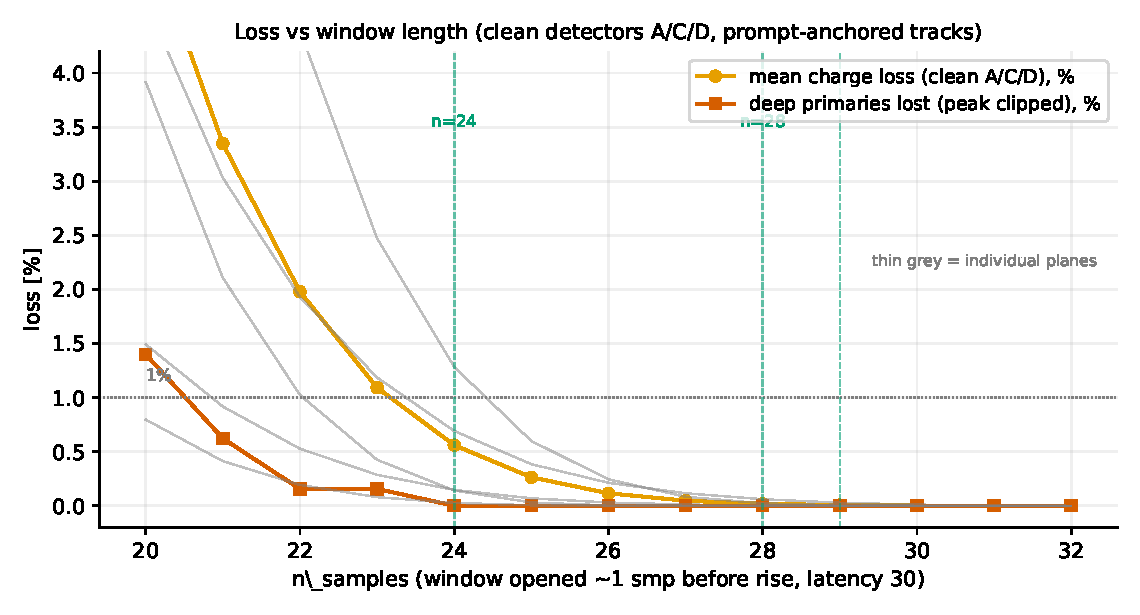
\includegraphics[width=\textwidth]{fig_loss_curve.pdf}
    \column{0.46\textwidth}\small
    Loss = measured pulse shape (charge vs truncation point) folded on the deep-edge
    distribution, prompt-anchored:
    \begin{itemize}\small
      \item \good{0 \% of primaries lost down to n=24} --- peaks are always captured; only the far charge \emph{tail} is clipped.
      \item mean charge loss \textbf{$<$0.6 \% to n=24}; steep knee below n$\approx$23.
      \item opening 1 smp before the rise costs a fixed $\sim$1 \% (anomalously early risers, likely not clean tracks).
    \end{itemize}
    \begin{center}\scriptsize
    \begin{tabular}{lccc}
      \toprule
      option & lat & n & cut \\\midrule
      conservative & 34 & 32 & 0 \\
      \good{balanced (now)} & 32 & 29 & 3 \\
      aggressive & 31 & 28 & 4 \\
      \bad{max-trim (B cleared)} & 30 & 24 & \textbf{8} \\
      \bottomrule
    \end{tabular}
    \end{center}
  \end{columns}
  \vspace{0.2em}
  \centering\small
  \bad{Gate = det B} (piles at smp 31): all but max-trim keep that bin. \textbf{Now: latency 32, n=29 (cut 3, $\sim$0 loss). After clearing B: latency 30, n=24 (cut 25\%, $<$0.6\% charge).}
\end{frame}

\begin{frame}{Det A: 600 $\to$ 700 V (staged) --- insurance, not speed}
  \begin{columns}[T]
    \column{0.55\textwidth}
    \textbf{Why}
    \begin{itemize}
      \item Today A is dry: 700 V buys only 0.7 smp. Irrelevant.
      \item \bad{The one catastrophic corner}: A@600 V in gas as wet as B/C/D \emph{already are} (0.8\%) $\Rightarrow$ 22.6 smp column $\Rightarrow$ truncates any affordable window (June's 500 V failure mode).
      \item A@700 V in the same gas: 17.7 smp $\Rightarrow$ fits n=28.
      \item A is first in the chain, but one flow drop / line disturbance makes it wet overnight.
      \item Physics cost $\approx$ nil (micro-TPC z-sampling $-$6\%).
    \end{itemize}
    \column{0.42\textwidth}
    \textbf{How (spark risk: sparked @800 V)}
    \begin{enumerate}
      \item one subrun at \textbf{650 V}, watch \texttt{hv\_monitor.csv} (trips, $I>0.2$ µA);
      \item then \textbf{700 V} soak under beam;
      \item fallback 650 V (still halves the wet-corner risk).
    \end{enumerate}
    \vspace{0.5em}
    B/C/D: keep 800 V --- wetter gas needs the field; nothing gained by lowering.
  \end{columns}
\end{frame}

\begin{frame}{Proposed on-beam drift scan (small, cheap, do it)}
  \begin{itemize}
    \item \textbf{det A only}: 600 V (reference exists) $\to$ 650 $\to$ 700, $\geq$30 min each during normal Mode-3 running. B/C/D untouched $\Rightarrow$ their physics data continues.
    \item Yields per point: $\sim$100--200 clean A-tracks/plane $\to$ span to $\pm$1 smp.
    \item Deliverables:
      \begin{enumerate}
        \item \textbf{spark/current stability at 650/700 = the actual gate} for the HV move;
        \item span(600)/span(700) ratio pins A's water content assumption-free (dry: 1.06, 0.8\%-wet: 1.28 --- cleanly separable);
        \item confirms the deep-edge + fall endpoint before freezing latency 34 / n=30.
      \end{enumerate}
    \item Optional, low priority: one B/C/D point at 750 V (wet-gas $v(E)$ slope); costs their margin while running.
  \end{itemize}
\end{frame}

\begin{frame}{v6 cross-check (done locally) --- A/C/D confirmed, det B flagged}
  \centering
  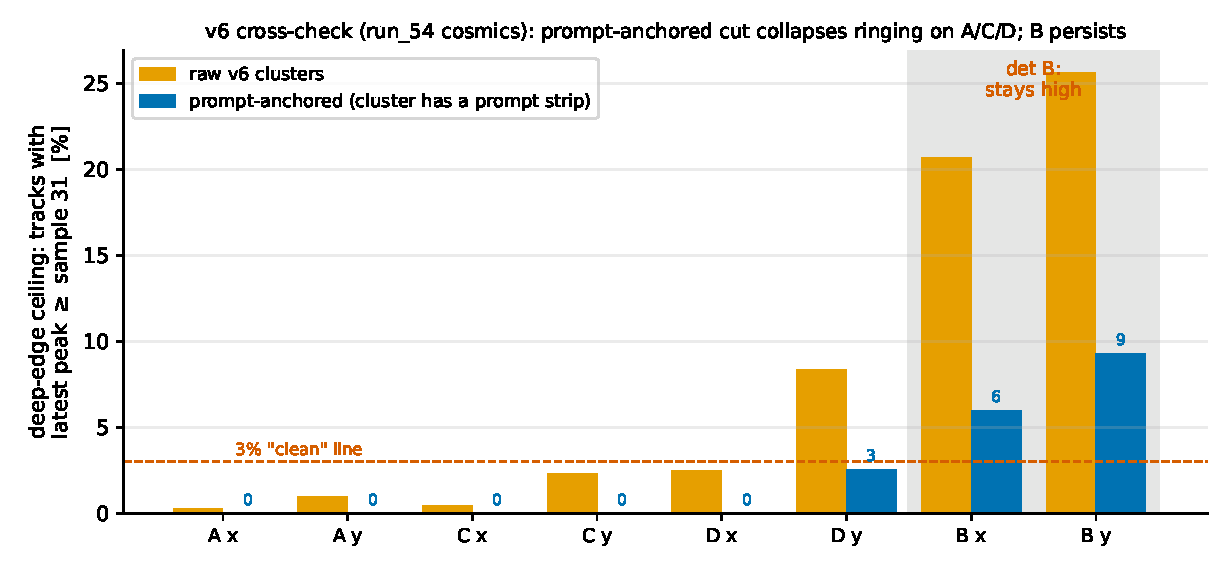
\includegraphics[width=0.86\textwidth]{fig_v6_crosscheck.pdf}
  \begin{columns}[T]
    \column{0.5\textwidth}
    \small\textbf{Prompt-anchored cut} (track cluster must contain a near-mesh strip, earliest $\leq$ smp 12) removes ringing clusters that lack one:
    \begin{itemize}\small
      \item \good{A, C, D collapse to 0--2.6\%} --- deep edges at smp 19--24, safely inside n=28. D$_y$'s 8.4\% was ringing, as predicted.
    \end{itemize}
    \column{0.5\textwidth}
    \begin{itemize}\small
      \item \bad{det B stays 6--9\%} at the smp-31 ceiling even anchored (span $\approx$20 $\to$ $v\approx$25 µm/ns). Small counts, cosmic-only.
      \item Either real slow drift (B wetter) \emph{or} residual coherent noise --- unresolved.
      \item \textbf{Impact:} B's fall rides the ceiling; \emph{clear B (noise vs slow-drift) or keep n=32} before the tightest trim.
    \end{itemize}
  \end{columns}
\end{frame}

\begin{frame}{Summary \& open items}
  \centering
  \begin{tabular}{ll}
    \toprule
    \textbf{knob} & \textbf{recommendation} \\
    \midrule
    latency & $35 \to \mathbf{32}$ now $\to \mathbf{30}$ after clearing B \\
    n\_samples & $32 \to \mathbf{29}$ now (cut 3, $\sim$0 loss) $\to \mathbf{24}$ after B (cut 25\%, $<$0.6\% charge) \\
    det A drift & $\mathbf{700}$ V, staged 650 $\to$ 700 with HV-monitor soak \\
    B/C/D drift & keep 800 V \\
    beam drift scan & yes --- det A 600/650/700, 30 min each \\
    \bottomrule
  \end{tabular}
  \vspace{0.8em}
  \begin{itemize}\small
    \item Loss priced from the \textbf{measured pulse} (rise $-$4, fall $+$7): 0\% primaries lost, $<$0.6\% charge to n=24 on clean dets. \bad{det B} (piles at smp 31) is the only gate to max-trim.
    \item v6 cross-check \good{DONE} locally (ROOT off-box; \textbf{never heavy jobs on the DAQ}): A/C/D clean, \bad{det B flagged}.
    \item Electronics follow-up: post-saturation ringing blocks (fixed per-FEU channel ranges); window trim already cuts most of it offline.
    \item Full writeup: \texttt{mx\_july\_beam\_qa/DRIFT\_WINDOW\_ANALYSIS.md} (\S6 = DAQ OOM incident).
  \end{itemize}
\end{frame}

\end{document}
